\documentclass[12pt]{report}
\usepackage[utf8]{inputenc}
\usepackage{titlesec}
\usepackage{geometry}
\usepackage{etoolbox}
\usepackage{xcolor}
\usepackage{enumitem}
\usepackage{amsmath}
\usepackage{xstring}
\usepackage{multicol}
\usepackage{tikz-dimline}
\usepackage{pdfpages}


% bibliography setup %
\usepackage[backend = biber,sorting = none]{biblatex}
\addbibresource{references.bib}

% appendix setup %
\usepackage{appendix}
\renewcommand{\appendixtocname}{Datasheets of all components}
\renewcommand{\appendixpagename}{Datasheets of all components}

% On the spot circuit creation %
\usepackage[american]{circuitikz}
\usepackage{tikz}
\usetikzlibrary{graphs}

% On the spot flowchart creation %
\usetikzlibrary{shapes.geometric, arrows}
\tikzstyle{startstop} = [rectangle, rounded corners, minimum width=3cm, minimum height=1cm,text centered, draw=black, fill=red!30]
\tikzstyle{io} = [trapezium, trapezium left angle=70, trapezium right angle=110, minimum width=3cm, minimum height=1cm, text centered, draw=black, fill=blue!30]
\tikzstyle{process} = [rectangle, minimum width=3cm, minimum height=1cm, text centered, draw=black, fill=orange!30]
\tikzstyle{arrow} = [thick,->,>=stealth]


% Image setup %
\usepackage{graphicx}
\graphicspath{{./images/}}

% Link setup %
\usepackage{hyperref}
\hypersetup{colorlinks=true, linkcolor=black, urlcolor=blue}


% caption layout for tables and images %
\usepackage{caption}
\usepackage{subcaption}
\captionsetup[table]{skip=7pt}
\captionsetup[figure]{skip=7pt}


% page layout %
\makeatletter
\patchcmd{\@makechapterhead}{50\p@}{75mm}{}{}
\patchcmd{\@makeschapterhead}{50\p@}{75mm}{}{}
\makeatother

\geometry{a4paper,left = 30mm,right = 20mm,top = 30mm,bottom = 22mm}
\textwidth = 160mm
\textheight = 245mm
\footskip = 7mm


% Paragraph and line spacing %
\setlength{\parindent}{12mm}
\setlength{\parskip}{2.5mm}


% title formatting %
\titleformat{\chapter}[block]{\Huge\bfseries}{Chapter \ \thechapter}{0.5ex}
{
    \rule{\textwidth}{0pt}
    \vspace{1ex}
    \centering
}
\titlespacing{\thechapter}{0mm}{12mm}{12mm}


% Section formatting %
\titleformat{\section}[hang]{\fontsize{16}{16}\bfseries}{ \thesection}{1.4em}{}
\titlespacing{\thesection}{}{15mm}{15mm}

% Subsection formatting %
\titleformat{\subsection}[hang]{\fontsize{14}{14}\bfseries}{ \thesubsection}{1.4em}{}
\titlespacing{\thesubsection}{}{15mm}{15mm}

% First level ordered list %
\setlist[enumerate,1]{label=(\alph*)}


\begin{document}


\includepdf[pages=-]{title_page}
\pagenumbering{roman}
\chapter*{Abstract}

A CNC based PCB Milling Machine incorporates the plan and usage of a CNC (Computer Numerical Control) machine to make PCB (Printed Circuit Board) in a particular set up. Creation of PCB within the present market is extremely costly when manufacture of testing circuits is taken into account. Along these lines, this CNC based PCB machine would be an efficient instrument through which circuit are often scratched and penetrated at an inexpensive rate. The creation of this CNC machine is to diminish the cost and multifaceted nature of machine. This venture manages the plan of a programmed scaled down CNC machine for PCB drawing and processing.  
A PCB Mill is a gadget that engraves out an example on a copper clad board with the end goal that it makes a Printed Circuit Board (PCB). PCBs are utilized in the field of electrical designing to interface electrical parts to each other.

 In CNC machine the program is put away in the memory of the system. The software engineer can easily compose the codes and alter the projects according to their necessities. These projects can be utilized for various parts and they don’t need to be rehashed once more. The CNC machine offers more prominent extra adaptability and computational ability. New frameworks and components can be joined into the CNC controller essentially by reconstructing the unit.
 
The CNC machine involves PC in which the program is sustained for cutting of the metal of the occupation according to the. All the slicing forms that are to be completed and all last measurements are encouraged into the PC through program. The PC hence realizes what precisely is to be done and does all the cutting procedures. CNC machine works like a Robot, which must be bolstered with the program and it takes after every one of your directions. A portion of the normal machine devices that can keep running on the CNC are: drilling machine or milling machine.

The principle motivation behind these machines is to expel a portion of the metal in order to give it appropriate shape, for example, round, rectangular and so on, the software guides the machine apparatus to perform different machining operations according to the program of guidelines sustained by the user, all the CNC machines are intended to meet close correctness.

The CNCs have tremendous advancement potential and many machining procedures can be communicated by methods for basic operations, for example interpretations, revolutions and by controlling the status of the CNC head. Numerous CNCs are controlled utilizing a unique programming dialect, named G-Code






\setcounter{page}{4}

\renewcommand*\contentsname{Table of Contents}
\tableofcontents

\listoffigures

\listoftables

\chapter{Introduction}
\thispagestyle{empty} % no page number for introduction

\setcounter{page}{2} % remember counting now starts from 2
\pagenumbering{arabic} % style changes back to arabic

\section{Project name and title}
The name of our project is CNC machine based complete PCB assembly line (milling).

\section{Problem statement}
Current factory-based PCB manufacturing targets large clients primarily for mass production. However, when it comes down to normal students, hobbyists, engineers mass production of PCBs is not what they expect. These small scale customers want fast but at the same time reliable and quality output for their products. \par

To solve the same this project attempts to create a CNC based PCB milling machine primarily for such small scale customers. Standard home-based PCB manufacturing techniques waste a considerable amount of time in the revelation of copper tracks on the PCB by sequential steps including (but not restricted to) UV exposure, etching, engraving, cleaning etc. till all tracks on a typical copper-clad are fully revealed. Although for PCBs of constant dimensions (which small scale clients usually prefer) each of the aforementioned steps takes on an average of 3 to 3.5 minutes time. \par

Hence, the total time required to develop a full PCB comes out to be 4 to 6 hours and may extend into multiple days if the concerned machines for the above processes are working under heavy load from other clients. This leads to a complete product delivery time in excess of 1-2 days (per PCB).


\section{Proposed solution}
It turns out that the processing time can be greatly reduced if we manage to target and reduce the time taken in those steps which are consuming a constantly large amount of time for every PCB irrespective of the design on it.  \par

Here the word design although a layman term refers to many things at once.
\begin{enumerate}
 \item The total number of tracks on the PCB
 \item The complexity in which the tracks are arranged amongst themselves
 \item The types of tracks (in terms of drill depth, length, thickness, clearance etc.)
\end{enumerate}

The time taken for the UV exposure process, etching process etc. are invariant of the design (word used in the same context as above) configuration of the PCB in terms of (a), (b) and (c). \par

A solution would be viable if we manage to directly engrave the tracks on a PCB as soon as the schematic file (.sch) or the board file (.brd) for a particular design is generated.In standard factory settings, if the above step is completed the PCB can proceed directly for drilling and component placement.However, the scope of our project is restricted to the successful completion of the former step in minimum time.



\section{Scope and report contents}
Chapter \ref{chapter2} starts with a critical analysis of the previous works that have been done using CNC machines including (but not restricted to) their applications in the PCB manufacturing industry. It goes on to discuss how every unit of the manufacturing process is done by optimal usage of CNC based processes. Added to that it also discusses few papers, journals as well as some commercial CNC instruction manuals. \par

Chapters \ref{chapter3} to \ref{chapter5} give a very detailed explanation of the current investigation. Chapter 3 deals with the manufacturing and construction of the CNC machine. Chapter \ref{chapter4} mostly deals with the main electronics and driving circuitry used in this project. While Chapter \ref{chapter5} details the reader on the software methodology and concludes the explanation of the current investigation. All the required steps are given sequentially in the order in which were carried out. \par

The final two chapters i.e. \ref{chapter6}  and \ref{chapter7} conclude with the findings of the current investigation, the logical results and analysis associated with it as well as give an insight into the future work plan of the project.

\chapter{Literature review} \label{chapter2}

\section{Review paper 1 - Prototype CNC machine design} 

\subsection{CNC Module introduction}
The Computer Numeric Control (CNC) \cite{ieee_pap} is a technology which aims to generate, parse and execute sequential action. It helps for the development of small and big sized CNC machines, based on a system with the capability of communication through a communication bus. It is also required electronic devices to run a CNC machine like controller circuit, as well, a software developed in LabVIEW to establish the communication between the machine and the computer. The objective of this work is the development of a machine which allows future use for PCB track designing with better efficiency than traditional methods.A CNC prototype machine was designed, with three-axis movement, with 300 mm of length both X and Y axes and 10 mm of the length Z-axis. \par

CNC Machines are often used in metal machining, like drilling, milling etc. This kind of machine consists usually of a servo mechanism controlled by a computer, a high-speed spindle and dedicated tools. This servo mechanism can be realized in a closed-loop fashion, using servo controllers driving DC or synchronous AC machines, or open-loop fashion, using stepper motors. small loads required an open-loop system for a better fit. Therefore, industrial-sized machines do not, in general, use open-loop machines. \par

The machine is based on the removal of the material of a workpiece. Nowadays, there are machines with six or more axes, which allow the machining of pieces which can handle high levels of complexity that is feasible by all other means.


\subsection{Use of CNC machine}
CNC machines can be used in many different ways, including (but not restricted to):

\begin{enumerate}
 \item Making circuits boards - They are used to make printed circuit boards for different products
 \item Making enclosures - The different types of CNC machines like laser cutters, mills and lathes use some parts to make enclosures. Sticker cutters are also used to make decorations for enclosures.
 \item For Computer Integrated Manufacturing - They are programmed in a specific way according to instructions, and this can save hundreds of thousands of hours of manual programming.
\end{enumerate}

The CNC machine is used in different industries, including:

\begin{enumerate}
 \item Agriculture - The agriculture industry requires reliable, high-quality production of machine parts and other products.
 \item Transportation - Some vehicle parts like gears, brakes, pins and shafts need precise CNC machining in their manufacturing.
 \item Firearms - CNC machines are needed to create complex barrels, plates and triggers, among other things.
\end{enumerate}

\section{Review paper 2 - Automatic mini CNC machine for drawing and drilling} 

\subsection{Methodology}
\cite{irjet_pap} The G code is interfaced with an Arduino CNC based controller by software which is used to convert into equivalent controller instructions. Hence it acts as an interfacing module between PC to Controller. This code is further passed to the stepper motor by easy drivers which convert the code and as per instructions the stepper motor moves. We need three axes X, Y, Z which operates as follows X stepper motor moves left and right Y stepper motor moves front and back and Z stepper motor up and down as per given dimensions these axes will move on.

\subsection{G codes and M codes}
PC G code is a converted instruction form of programming language which defines instructions on where to move, how fast to move with the path.

\subsection{CNC shield}
\begin{itemize}
 \item GRBL 0.8c compatible. (Open supply microcode that runs on associate degree Arduino UNO that turns G-code commands into stepper signal.)
 \item 4-Axis support (X, Y, Z, A which can duplicate X, Y, Z or do a full 4th axis with custom firmware using pins D12 and D13)
 \item 2 x finish stops for every axis (6 in total)
 \item Spindle enable and direction
 \item Coolant enable
 \item Uses removable Pololu A4988 compatible stepper drivers. (A4988, DRV8825 and others)
 \item Jumpers to line the Micro stepping for the stepper drivers. (Some drivers just like the DRV8825 will do up to 1/32 micro-stepping )
 \item Compact design
 \item Stepper Motors may be connected with four pin Molex connectors.
 \item Runs on 12-36V DC. (At the instant solely the Pololu DRV8825 drivers will handle up to 36V thus please take into account the operation voltage once powering the board.
\end{itemize}

\subsection{Generic block diagram}

\begin{figure}[h]
 \centering
 \includegraphics{Chapter_2/paper_block_diagram.png}
 \caption{Block diagram of the CNC machine developed in the paper}
 \label{fig:block_diagram}
\end{figure}

\subsection{Stepper motor and associated parts}

\subsubsection*{NEMA 17 stepper motor}
Stepper motors are sort of DC motors that move in increments or steps, they move at a legendary interval for every pulse of power. These pulses of power are provided by a motor driver and are referred to as a step. As every step moves a legendary distance it makes them handy devices for repeatable positioning. Stepper motors are usually used on CNC Machines such as 3D Printers, Laser Cutters, CNC Routers.


\subsection{Micro controller requirements}

\subsubsection*{Micro controller - Arduino UNO r3}
The Arduino UNO R3 could be a microcontroller board supporting the ATmega328. It has fourteen digital input/output pins (of that vi may be used as PWM outputs), 6 analog inputs, a 16 MHz crystal oscillator, a USB connection, a power jack, an ICSP header, and a reset button. It contains everything required to support the microcontroller; merely connect it to a PC with a USB cable or power it with an AC-to-DC adapter or battery to induce power. \par

The Uno differs from all preceding boards in that it doesn't use the FTDI USB-to-serial driver chip. Instead, it options the Atmega16U2 (Atmega8U2 up to version R2) programmed as a USB-to-serial converter.
Revision a pair of the Uno board features a resistance propulsion the 8U2 HWB line to ground, making it easier to put into DFU.

Revision three of the board has the subsequent new features:

\begin{itemize}
 \item Added SDA and SCL pins that are near to the AREF pin and 2 other new pins placed near the RESET pin, the IOREF that allow the shields to adapt to the voltage provided from the board. In future, shields are compatible with the board that uses the AVR, which operates with 5V and with the Arduino Due that operate with 3.3V. The other could be a not connected pin, that is reserved for future functions.
 \item Stronger RESET circuit.
 \item Atmega 16U2 replaced the 8U2.
\end{itemize}


\section{Review paper 3 - CNC fabrication and user manual} \label{Sec:3} 

This reference \cite{iiit_pap} instead of being a paper happens to be a detailed user manual regarding how one should use a typical CNC machine for PCB prototyping purposes. It starts on similar lines of needs and requirements as the CNC machine being developed by the authors of this report. It then goes on to explain various software aspects of PCB design followed by which it describes what are the standard and special procedures used in CNC machines such as moving the tooltip to the origin/soft - home position, calibration of various important parts to name a few. \par

A BYO PCB prototyping machine capable of developing both through hole and Surface Mount Technology on single sided and double sided PCB boards has been used as a standard reference throughout the manual. Following is a detailed description of  only the important and relevant sections of the concerned manual.


\begin{figure}[h]

 \begin{subfigure}{0.5\textwidth}
  \includegraphics[width=0.9\linewidth, height=6cm]{Chapter_2/mechanical_setup.PNG}
  \caption{Mechanical Setup of the Machine}
  \label{fig:subim1}
 \end{subfigure}
 \begin{subfigure}{0.5\textwidth}
  \includegraphics[width=0.9\linewidth, height=6cm]{Chapter_2/electronics_assembly.PNG}
  \caption{Electronics hardware assembly}
  \label{fig:subim2}
 \end{subfigure}

 \caption{The PCB prototyping machine as described in the reference manual}
 \label{fig:paper_cnc_machine}
\end{figure}


\subsection{Layers of a PCB copper clad}

Understanding PCB composition in hindsight is simply understanding how layers of a PCB are stacked over one other and what is the significance of each layer. The most important layer(s) of the PCB copper cladding is the copper layers themselves. These are the layers through which the intended electrical signals pass depending on the application. The copper layers sandwich a layer which is usually the thickest layer in a copper cladding. It is an insulating layer called the substrate. Depending on the application the substrate layer could be made of various materials of various thicknesses. The most common ones are FR4 which is a NEMA grade designation for glass-reinforced epoxy laminate material and FR2 which is a phenolic cotton paper. FR2 is very common in single-sided PCBs in consumer electronics while FR4 is universal in multi-layer PCBs and in general. \par


\begin{figure}[h]
 \centering
 \includegraphics{Chapter_2/pcb_layers.PNG}
 \caption{The layers of a double-sided PCB}
 \label{fig:pcb_layers}
\end{figure}

Now to insulate and protect the copper layers they are covered by a thin lacquer-like material called the solder mask. This layer is responsible for the characteristic “green” colour of PCBs or whatever colour (red, blue etc.) they are supposed to have. Then the final set of top and bottom layers of a PCB is the silkscreen which has a look and feels similar to ink and can be used to add texts and logos to a PCB. Following is an illustration of the various layers of a double-sided PCB copper cladding. \par

% add table for eagle layers %


The PCB designer has access to all the layers at any given instant of time during the development of a particular PCB. For the designer using the EAGLE software, a palette of colours (as shown below) is used to represent the various layers of a PCB. They can be toggled according to the convenience of the designer by going into the layer settings of the board and clicking the layer number to toggle it in view.

\subsection{CAM processing}

CAD/CAM processing belongs to a much larger set/group of processes used in the industry collectively called machining. \textbf{Machining} is any of the varied processes during which a bit of staple is dug into a desired final shape and size by a controlled material removal process. The common theme of machining remains as controlled material removal which could be either additive or subtractive. As the words themselves suggest additive manufacturing shall add material to the original raw material while subtractive manufacturing refers to the opposite.  \par

Nowadays, all machining has been converted into OR is exclusively carried out by Computer Numerical Control (CNC). Computer-Aided Design (CAD) and Computer-Aided Manufacturing (CAM) fall under this much larger umbrella of  “CNC jobs”. This paper explains how to use the CAM processor present in the EAGLE software to generate a CNC job corresponding to a given board file. The same CAM processor can be used to generate  “Gerber” files for all the layer(s) of a given PCB as well as “Excellon” files for drilling purposes of the concerned  PCB. These types of files come under the much larger umbrella of PCB NC formats which manage to convey routing and drilling information to the concerned CNC machine. \par

Later the Gerber files generated are sent to “FlatCAM” which is a CAM processing software responsible for generating CNC jobs from Gerber files obtained from any PCB CAD program. It does the additional job of generating corresponding “g codes” for routing purposes and allowing the user to edit the same.


\subsection{Special procedures} \label{spec_proc}

Several challenges arise when designing complex PCB designs; these challenges could range from manufacturing multilayered boards to working on uneven surfaces. The associated software for a given CNC machine and some simple procedures help the users overcome these challenges. Few of those which were discussed in this paper are described below.

\subsubsection*{Auto levelling}
It is not uncommon to have inconsistent traces in larger PCBs while using a CNC based milling machine. Such inconsistencies arise due to minor height variations of the surface on which the PCB is kept (“wasteboard”) OR the PCB by itself could be bent or warped. It should be noted that even minor height variations of about 1 mm could change the groove width by about 0.672 mm.  To overcome this problem we need specialised software called auto levelling software. By definition, Auto-levelling is a process that tries to \textbf{compensate} for height differences instead of \textbf{trying to prevent them.} \par

Auto levelling software depending on their sophistication may approach this problem in different ways and use different forms of sensory data to solve the problem. The most common way to approach this problem is by dividing the entire PCB into uniform geometrical grids. This gives specific sampling positions which could be probed to get an overall idea of the non-uniformities of the surface. E.g. a 40 x 40 mm surface could be divided into 100 grids of 4 x 4 mm and the surface at the centre of the grids is always probed.  Probing the height of a PCB locally (i.e. in every grid) is typically done by slowly lowering an end mill until an \textbf{electric connection is made between the end mill and board’s copper layer}. All these things are usually automated by the software. However, if it is not the case the designer has to design compensation algorithms on their own. \par

First, all the collected data is accumulated in a single file called the probe file. The generated G code and this file are superimposed and fed to the software. The software now tries to fit a \textit{quadratic surface} (say of the form $f(x^{2},y^{2})$) on the probe data and accordingly adjusts the G code in the vertical direction. This adjusted G code can be fed into the CNC machine like any other G code file thereby eliminating any problems that may result from an uneven or warped surface.

\begin{figure}[h]
 \centering
 \includegraphics{Chapter_2/with_and_without_autolevel.PNG}
 \caption{Showing the making of PCB board with and
  without the use of Autoleveller on a skewed platform}
 \label{fig:with_without_auto}
\end{figure}

\subsubsection*{Copper area clear}

With RF circuit PCBs or any PCB, in general, comes the problem of clearing large areas of unwanted copper traces which is just unwanted core load. The manual explains how to use the various properties available under the “Gerber object” tab to eliminate unwanted copper traces. After specifying the margin dimensions, a boundary (called the “bounding box”) is created. A geometric subtraction of the Gerber object from the boundary will give rise to another Gerber object which doesn’t have areas with copper on them. Several polygons constitute this newly formed Gerber object. The user gets to choose which Gerber object to keep and what not to. To do so the correct tool dimensions with its specifications are selected and the concerned/desired polygon is painted. “Painting” refers to covering the whole polygon with the tool paths (whose specifications were selected within the previous step). In this manner, all unwanted copper load can be removed from any type of PCB.

\begin{figure}[ht]
 \begin{subfigure}{0.5\textwidth}
  \includegraphics[width=\linewidth, height=6cm]{Chapter_2/copper_area_clear_1.PNG}
  \caption{Geometry object with polygons covering the areas without copper}
  \label{fig:copper_clear_1}
 \end{subfigure}
 \begin{subfigure}{0.5\textwidth}
  \includegraphics[width=0.9\linewidth, height=6cm]{Chapter_2/copper_area_clear 2.PNG}
  \caption{New Geometry Object with the desired tool paths that can overlap too.}
  \label{fig:copper_clear_2}
 \end{subfigure}

 \caption{The software steps during the procedure of \textit{copper clear}}
 \label{fig:copper_clear}
\end{figure}

\subsubsection*{Board cutout} \label{outline_cut}

PCBs need to be cut out from much larger and blank copper claddings, otherwise, we shall incur large material wastage in terms of area and cost. The FlatCAM software allows the user to do so by selecting the board cutout tab after choosing a Gerber file. The desired margin (dimension) is selected which tells how far the cutout boundary is from any element of the Gerber source of the PCB. After this “gaps” can be selected for the cutout in terms of their dimensions and their number. It is always recommended to have gap size twice the diameter of the tooltip. FlatCAM allows two gaps (either on top and bottom OR left and right) or four gaps for a given PCB. Once, this step is complete, just like the previous procedure the geometry for the tool path is generated. A CNC job is created from this geometry just like any other geometry and now the job is ready to be processed.  Hence, this feature allows precise cutting of a PCB from its larger blank cladding once the main CNC job is done.

\begin{figure}[h]
 \centering
 \includegraphics{Chapter_2/board_cutout.PNG}
 \caption{Typical CNC job corresponding to a \textit{board cutout}}
 \label{fig:board_cutout}
\end{figure}


\subsection{Computing resolution and accuracy} \label{res_and_acc}
A lot of experimentation needs to be carried out to verify the practicality of the CNC machine. A typical experimentation procedure needs to be carried out to find out the wire width and resolution capabilities of the PCB. The next part is computing the resolution for SMT fabrication purposes. Both the techniques have been briefly discussed in the manual.

\subsubsection*{Computing wire width and resolution}
To find out the level of resolution while tracing out or engraving wires, a good way is to make a very simple PCB consisting of wires of various widths, to be precise, in decreasing order. The wire of largest possible width (available in the schematic design software) is made followed by the next largest and so on until the wire of minimum possible width possible in the schematic design software is designed. Now the G codes corresponding to this sample PCB are sent to the CNC machine before milling the same. \par

After the PCB tracks have been engraved on to the copper cladding by the CNC machine, the absolute deviation between the width of the actual engraved tracks and input width for the concerned track provided as input from the software is computed. (Insert equation) This denotes the resolution of the CNC machine. It should be noted that it is not compulsory to compute the absolute deviation, positive and negative deviations are both valid. To carry out this measurement, a handheld microscope is a suitable instrument. For the CNC machine in question, the wire of the smallest width that could be fabricated was found out to be 0.2 mm with an allowable deviation of -0.012 mm.

\begin{figure}[h]
 \centering
 \includegraphics{Chapter_2/test_widths.PNG}
 \caption{PCB fabricated with sample wires of varying widths}
 \label{fig:wire_widths}
\end{figure}


\subsubsection*{Resolution of SMT}

Various standard and commonly used SMT packages were fabricated by the CNC machine. It was found out that the minimum pitch size of an SMT that could be fabricated was about as low as 0.3 mm. A handheld USB microscope was used for measurements in each case.

\begin{figure}[h]
 \centering
 \includegraphics{Chapter_2/test_smt.PNG}
 \caption{PCB fabricated with SMTs of varying footprints}
 \label{fig:smts}
\end{figure}

\chapter{Construction and Manufacturing} \label{chapter3}

\section{Base material} \label{bmaterial}

To accurately describe the expected dimensions of this base material it is important to know the target PCB size for the concerned CNC machine since along with the required machinery and hardware that would be mounted on the base material, the PCB is the main working component. For this project the designers have targeted \textbf{15 cm x 15 cm single sided copper clad PCBs}. \par

It is obvious that the net dimensions of the base material would need to be greater than that of the target PCB size. After performing multiple calculations as described in the following sections. The final base material size has been fixed at \textbf{40 cm x 40 cm}.

\begin{figure}[h]
 \centering
 \begin{tikzpicture}[scale=0.2]
  \draw (0,0) rectangle (40,40);
  \draw [blue] (0,0) rectangle (15,15);
 \end{tikzpicture}
 \caption{Drawing showing maximum PCB dimensions that can be manufactured (in \textcolor{blue}{blue}) superimposed on base material dimensions represented on a $1:5$ scale}
 \label{fig:base}
\end{figure}


\section{XY axes made up of normal unpolished wood}

The two segments of wood which must have the primary load bearing capacity are the XY axes. The X segment consists of a wooden plank like structure with slots of length $15$ mm and depth $8$ mm each to insert wooden blocks on it. A similar structure exists for Y - axis segment as well. Dimensions for both the segments are illustrated below. \par

\begin{figure}[h]
 \begin{center}
  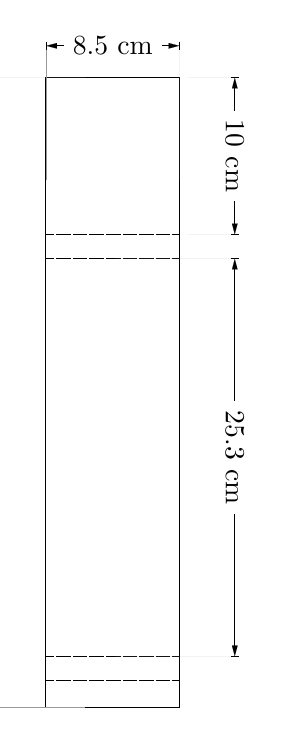
\begin{tikzpicture}[scale=0.2]
   \draw (0,0) rectangle (8.5,40);
   \draw [dashed] (0,1.7) rectangle (8.5,1.7);
   \draw [dashed] (0,3.2) rectangle (8.5,3.2);
   \draw [dashed] (0,28.5) rectangle (8.5,28.5);
   \draw [dashed] (0,30) rectangle (8.5,30);
   \hspace{-15mm}
   \dimline [extension start length=0.25, extension end length=0.25, line style = {line width=0.5}]{(0,0)}{(0,40)}{40 cm};
   \hspace{15mm}
   \dimline[line style={line width=0.5},extension start length=1,extension end length=1]{(0,42)}{(8.5,42)}{8.5 cm};
   \dimline[line style={line width=0.5},extension start length=0.3,extension end length=0.3]{(12,40)}{(12,30)}{10 cm};
   \dimline[line style={line width=0.5},extension start length=0.3,extension end length=0.3]{(12,28.5)}{(12,3.2)}{25.3 cm};
  \end{tikzpicture}
 \end{center}
 \begin{center}
  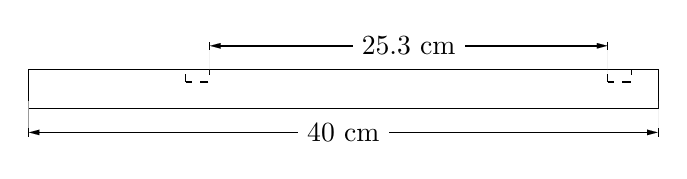
\begin{tikzpicture}[scale=0.2]
   \draw (0,0) rectangle (40,2.5);
   \draw [dashed] (10,1.7) rectangle (11.5,2.5);
   \draw [dashed] (36.8,1.7) rectangle (38.3,2.5);
   \dimline[line style={line width=0.5},extension start length=0.07,extension end length=0.07]{(11.5,4)}{(36.8,4)}{25.3 cm};
   \dimline[line style={line width=0.5},extension start length=-0.05,extension end length=-0.05]{(0,-1.5)}{(40,-1.5)}{40 cm};
  \end{tikzpicture}
 \end{center}
 \caption{(From top to bottom) Top view and front view of the X-axis segment with dimensions represented on a $1:5$ scale}
 \label{fig:xaxis}
\end{figure}

Following page shows the structure of the Y - axis segment which has a similar scheme of construction but with slightly reduced dimensions. \pagebreak

\begin{figure}[h]
 \begin{center}
  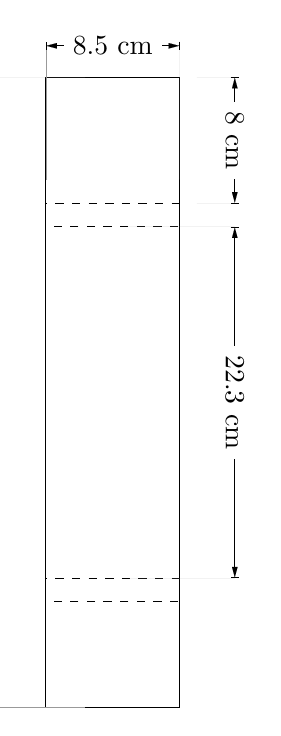
\begin{tikzpicture}[scale=0.2]
   \draw (0,0) rectangle (8.5,40);
   \draw [dashed] (0,6.7) rectangle (8.5,8.2);
   \draw [dashed] (0,30.5) rectangle (8.5,32);
   \hspace{-15mm}
   \dimline [extension start length=0.25, extension end length=0.25, line style = {line width=0.5}]{(0,0)}{(0,40)}{40 cm};
   \hspace{15mm}
   \dimline[line style={line width=0.5},extension start length=1,extension end length=1]{(0,42)}{(8.5,42)}{8.5 cm};
   \dimline[line style={line width=0.5},extension start length=0.3,extension end length=0.3]{(12,40)}{(12,32)}{8 cm};
   \dimline[line style={line width=0.5},extension start length=0.3,extension end length=0.3]{(12,30.5)}{(12,8.2)}{22.3 cm};
  \end{tikzpicture}
 \end{center}
 \begin{center}
  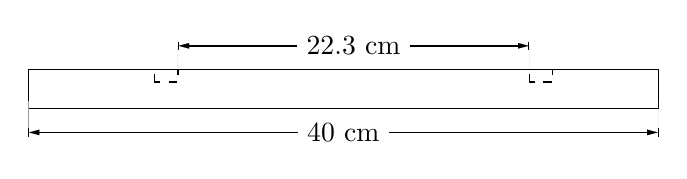
\begin{tikzpicture}[scale=0.2]
   \draw (0,0) rectangle (40,2.5);
   \draw [dashed] (8,1.7) rectangle (9.5,2.5);
   \draw [dashed] (31.8,1.7) rectangle (33.3,2.5);
   \dimline[line style={line width=0.5},extension start length=0.07,extension end length=0.07]{(9.5,4)}{(31.8,4)}{22.3 cm};
   \dimline[line style={line width=0.5},extension start length=-0.05,extension end length=-0.05]{(0,-1.5)}{(40,-1.5)}{40 cm};
  \end{tikzpicture}
 \end{center}
 \caption{(From top to bottom) Top view and front view of the Y-axis segment with dimensions represented on a $1:5$ scale}
 \label{fig:yaxis}
\end{figure}

The motor resides behind one block (say $B_{1}$) while the block on the other end is idle (say $B_{2}$). The face of $B_{1}$ which faces $B_{2}$ has two holes drilled in it. The guide rod connected to the motor shaft is inserted into the larger hole while the support rod is inserted into the smaller hole. The respective dimensions of the hole are clearly mentioned in the diagram and are identical for both $B_{1}$ and $B_{2}$. \par

Additionally as mentioned before dimension buffers are always necessary. The buffer which has been used here (both for $B_{1}$ and $B_{2}$) is: the center of the smaller hole is located at a distance of 1.5 cm from the left end while the center of the larger hole is 3 cm from the right end. The overall buffer which was available at the end for the two blocks were
(Left buffer $-$ radius of smaller hole) $+$ (Right buffer $-$ radius of larger hole)
$= (1.5 - 0.6) + (3 - 1.65)
 = 0.9 + 1.35
 = 2.25$ cm \par

The block $B_{2}$ as mentioned earlier is idle - the face of the block which does not face $B_{1}$ is fully empty. And the sole purpose of $B_{2}$ is to stabilise other ends of the main guide rod as well as the support rod. This is accomplished by the bearing arrangements made on the face facing the concerned face of $B_{1}$ as mentioned earlier. Details of the bearing design and the means through which they become compatible with the wooden block faces and the concerned guide or support rods are mentioned in the subsequent sections.

\begin{figure}[h]

 \begin{subfigure}{0.5\textwidth}
  \hspace{8mm}
  \includegraphics[width=0.8\linewidth, height=6cm]{Chapter_3/B1.png}
  \caption{Block $B_{1}$}
  \label{fig:b1}
 \end{subfigure}
 \begin{subfigure}{0.5\textwidth}
  \hspace{8mm}
  \includegraphics[width=0.8\linewidth, height=6cm]{Chapter_3/B2.png}
  \caption{Block $B_{2}$}
  \label{fig:b2}
 \end{subfigure}

 \caption{Three - dimensional representation of wooden blocks $B_{1}$ and $B_{2}$ with all the relevant dimensions and annotations (not to scale)}
 \label{fig:b1b2}
\end{figure}


\section{Guide rod and complementary support rods}

A pair of guide rod and complementary support rods are required for the XY axes. Before proceeding further it should be noted that the guide rod is threaded while the support rod is smooth. The threaded rod is made up of mild steel while the smooth rod material is stainless steel. As per design specifications, these rods must run perfectly parallel to each other. Ensuring the same is a critical design challenge. \par

The length of the threaded rod for the X- axis segment is 30 cm while for the Y- axis it comes out to be 27.5 cm. Further, there is no proper specification for the smooth rod lengths rather a larger sized ready made rod is cut to a length so that it fits between the blocks $B_{1}$ and $B_{2}$ (with all other dimensions taken into consideration). \par

However, although the rod (threaded) lengths are non identical, the thread pitch, the hole (to be drilled on the motor shaft end) specifications and the diameter are exactly identical. The thread pitch was decided at 1.25 mm. Since the rod on both ends will be held by smooth bearings, some part of the threading on both ends need to be removed. From the shaft side the threading has been deprecated by 3.3 cm while on the other end the threading has been reduced by 1.3 cm. The original diameter of the threaded rod was 1.2 cm however due to the thread deprivation on both sides the diameter has reduced to 1.0 cm on both ends for the concerned amount of thread deprived lengths. For the hole on the shaft side: the drill depth must be exactly equal to the shaft length with zero buffer. The shaft length is 2.3 cm and hence it is the drill depth as well. The diameter of the drill hole is fixed at 5 mm. Another hole must be drilled perpendicular to the rod axis at a distance of 1 cm from the shaft end. A fastening screw shall pass through this hole intersecting the motor shaft axis at a right angle.

% Show to scale image of the guide rod and complementary support rods one below the other %


\section{Bearing design}

As stated in the previous section it is obvious that a total of four bearings are needed: one on both ends of threaded rods of both the axes. Metal bearings in the manufacturing industry are specified by their inner diameters. Small spherical balls line up the space between the inner diameter and the outer diameters. These spherical balls reduce friction while the threaded rod rotates under the actuating action of the motor. These spherical balls are the actual bearings where the name of this machine part has come from. \par

In our project the inner diameter of the bearing is 1.0 cm (matching with the thread deprived rod diameter as mentioned in the previous section) while the outer diameter of the same comes out to be 3.3 cm.

\begin{figure}[h]
 \centering
 \includegraphics[scale = 0.5]{Chapter_3/bearing.PNG}
 \caption{Metal bearings similar to the ones used in the project}
 \label{fig:bearing}
\end{figure}

\section{Roller wheel section}

One end of the Y-axis (Wooden structure) is rested on top of the X-axis, while the other end is freely hanging. This might cause the Y-axis to lean towards that end. In order to make sure that the axis is stable, we have used a “ball castor wheel” which is attached to the free end of the Y-axis. This helps the axis to be perpendicularly aligned with X-axis and aligned in parallel with the base. To attach the wheel to the Y-axis we have made a wooden block which is of sufficient height to align the axis parallel to the base.

\begin{figure}[h]
 \centering
 \includegraphics[scale = 0.32]{Chapter_3/ball_castor.jpeg}
 \caption{A set of castor wheels with a rubber endings similar to the one used in the project}
 \label{fig:ballcastor}
\end{figure}

\section{Engraving bits' selection}

The most important part of the CNC machine is the tooltip and its material constituents. The tooltip in case of our CNC machine is an engraving bit made of Tungsten Carbide. In general, such bits are expensive for either engraving or drilling applications. However, they are quite invaluable and universal in nature for almost all CNC based applications. For a CNC based PCB milling machine, a lot of attention is paid on the dimensions of the engraving bit because it directly corresponds to the accuracy of the system. For PCB milling purposes the minimum dimensions of the engraving bit that was purchased were 0.7 mm while the largest measured at about 3.2 mm. Following is an illustration of an engraving bit with all the relevant dimensions that would help the designer choose an appropriate size for a given set of specifications.

\begin{figure}[h]
 \centering
 \includegraphics[scale = 0.75]{Chapter_3/engrav_bit.PNG}
 \caption{An illustration of a Tungsten Carbide engraving bit with all the relevant dimensions}
 \label{fig:ebit}
\end{figure}

\section{Coupling and fastening screws} \label{screws}
These two types of screws are required in abundance throughout the mechanical assembly for either fixing components to their respective base(s) of different materials OR to join/fix simultaneously actuated (usually) components. Now the primary parameter deciding screw specifications is material thickness on which the screw shall impinge. \par

For fastening screws impinging on the base or the plank material 1.5 mm screws are sufficient. For coupling screws, used only in one application: secure coupling of threaded rod and motor shaft, a specification of 3 mm is sufficient.

\begin{figure}[h]
 \centering
 \includegraphics[scale = 0.59]{Chapter_3/coupling_screw.png}
 \caption{A coupling screw with all the relevant dimensions and similar to the ones used in the project}
 \label{fig:cscrew}
\end{figure} \pagebreak

\begin{figure}[h]
 \centering
 \includegraphics[scale = 0.59]{Chapter_3/fastening_screw.png}
 \caption{A fastening screw with all the relevant dimensions and similar to the ones used in the project}
 \label{fig:fscrew}
\end{figure}

\chapter{Electronic and driving circuitry} \label{chapter4}

\section{Power supply} \label{psupply}

In our project, there are three major electronic components which have different power ratings. We have to power an Arduino UNO board, portable mini electric drill and a CNC shield. The Arduino UNO board are often powered via the USB connection or with an external power supply. The power source is selected automatically. External (non-USB) power can come either from an AC-to-DC adapter or battery. The adapter is often connected by plugging a 2.1mm centre-positive plug into the board's power jack. Leads from a battery are often inserted within the GND and Vin pin headers of the source connector. The board can operate an external supply from 6 to 20 volts. If furnished with but  7V, however, the 5V pin could provide but five volts and therefore the board may become unstable. If using quite 12V, the voltage regulator may overheat and damage the board. The recommended range is 7 to 12 volts. The current requirement ranges from 1A - 3A. \par

On the other hand, the electric drill comes in with an attached AC/DC adapter which has an output rating of 9V/1A and is sufficient to rotate the drill bit at nominal speeds. The drill also has manual control for the drill speed (in rpm) which internally adjusts a potentiometer to get the required speed. Similarly, the CNC shield has a rated voltage requirement of 12 - 36 VDC. Now, the problem is to come up with a single (if possible, customised) Power Supply Unit (PSU) which can handle all the devices at once. The 9V rated AC/DC adapter in the electric drill is sufficient to power the Arduino UNO board although it is not even barely sufficient to power the CNC shield (let alone after the current calibration process). At the same time, the current rating of the drill is unknown. Assuming the current rating is in the neighbourhood of 1A (same as the output of the complementary adapter) then splitting its output wires won’t help because the Arduino board won’t receive the expected current for its stable or nominal operation (even if we assume it works in the neighbourhood of the lower bound of the range 1A-3A). These conditions imply that developing a customised PSU for the entire system is very difficult. Even if we use an AC/DC adapter which has a voltage rating of 9V - 12V and a current rating of 1A - 5A with separated output lines it would simply manage to power the Arduino UNO and the electric drill but not the CNC shield. It implies that an adapter having a voltage rating somewhere near 24V will suffice but separate resistors would need to be used (preferably in a voltage divider network) to provide reduced voltage supply to the Arduino UNO board. \par

However, it should be noted that no customised PSU was developed for this project nor were these two electronic components powered by the same unit. The Arduino UNO development board was powered via the USB connection from a laptop while the drill was used along with its complementary AC/DC adapter without any modifications. The CNC shield, on the other hand, was directly powered from a DC regulated power supply.

\begin{figure}[h]
 \begin{center}
  \begin{subfigure}{0.5\textwidth}
   \includegraphics[width=\linewidth, height=6cm]{Chapter_4/dual_dc_regulated_power_supply.jpg}
   \caption{Dual DC regulated power supply rated at 30V/2A for powering the CNC shield}
   \label{fig:dc_supply}
  \end{subfigure} \\
 \end{center}

 \begin{subfigure}{0.5\textwidth}
  \hspace{5mm}
  \includegraphics[width=0.9\linewidth, height=6cm]{Chapter_4/arduino_power.png}
  \caption{The Arduino UNO board being powered by USB supply from a laptop}
  \label{fig:arduino_supply}
 \end{subfigure}
 \begin{subfigure}{0.5\textwidth}
  \includegraphics[width=0.9\linewidth, height=6cm]{Chapter_4/adapter.jpg}
  \caption{An AC-DC adapter rated at 9V/1A used for powering the electric drill}
  \label{fig:ac_dc_adapter}
 \end{subfigure}

 \caption{Various distinct power supplies used in the project}
 \label{fig:power_supplies}
\end{figure}

\section{CNC motors}

The most important part of this project is the CNC shield and associated motors. Our project consists of three axes (X-axis, Y-axis and Z-axis) which are controlled by two stepper motors (for X and Y axes) and a single servo motor (for vertical movement of drill bit i.e. Z-axis).

\subsection{Stepper motors} \label{step_motors}

Both X and Y axes are independently controlled by NEMA 17 stepper motors so we require two stepper motors in this project. The stepper motor assigned for the X-axis segment must be able to rotate a coupled rod, resting on which is the entire Y-axis segment (a part of whose weight is resting on this threaded rod and another smooth support rod). So a large capacity stepper motor needs to be considered. If possible, going for a larger capacity stepper motor (say NEMA 23) for the X-axis would ease out the operations in terms of fast and precise movement. \par

The stepper motor for the Y-axis segment is relatively less constrained in terms of weight capacity and any suitable capacity motor which can rotate a threaded rod will do. The NEMA 17 stepper motors used for this project are bipolar i.e. there is only a single winding per phase. The driving circuit must be more complicated to reverse the magnetic pole, this is often done to reverse the current in the winding. However, all that complexity is handled by the dedicated drivers onboard the *CNC shield*. Following is an illustration of the motor (identical to the one used in the project) followed by a table of its summarised electrical and mechanical specifications.

\begin{figure}[h]
 \centering
 \includegraphics[scale=0.2]{Chapter_4/nema_17.jpg}
 \caption{NEMA 17 stepper motor similar to the one used in the project}
 \label{fig:stepper}
\end{figure}

%  table of brief specifications %


\subsection{Servo motor}

The only function of the servo motor of Z-axis is to produce minimal linear actuation of the drill bit (which is attached to the electric drill at its bottom) along the positive and negative Z-axis. Such type of behaviour may be seen when the CNC machine moves from one milling position to another by moving over non-processable space or area on the PCB. For this, we have used a servo motor which can raise the drill bit with gear precision. In terms of G code following is a sample self-explanatory code which may lead to such a movement of the Z-axis.


\begin{flushleft}
 {\fontfamily{qcr}\selectfont G91 (use relative positioning) \\
  G1 Z10 (move z-axis up by 10 mm) \\
  \hspace{18.2mm}(irrespective of initial position)
 }
\end{flushleft}

It should be noted that there are many other equivalent instructions which would produce the same linear actuation. Depending on what the *software* determines to be feasible in terms of time and space, the appropriate set of G code(s) would be used at the concerning point in the operation of the CNC machine. Following is an illustration of the motor (identical to the one used in the project) followed by a table of its summarised electrical and mechanical specifications.

\begin{figure}[h]
 \centering
 \includegraphics[scale=0.4]{Chapter_4/servo.jpg}
 \caption{Gear precision servo similar to the one used in the project}
 \label{fig:servo}
\end{figure}

%  table of brief specifications %

\section{Micro controller}

The use of a microcontroller for this specific project is to read the G codes and M-codes and interpret it into corresponding pulses to run the motors. Thus the microcontroller to be used can be of basic specifications. However, it should be noted that the CNC shield should be compatible with the microcontroller development board being used. At the same time, the total cost of the board and the shield shouldn’t exceed the budgetary requirements of the project. \par

Depending on the above conditions we have used an Arduino UNO which is based on ATmega328 microcontroller. A compatible shield for this board is also available in the market. It has 14 digital I/O pins(out of which 6 can be used as PWM outputs and hence major significance in this project), 6 analog inputs and a 16 MHz ceramic resonator (CSTCE16M0V53-R0), a USB connection, an influence(power) jack, an ICSP header, and a reset button. It basically contains everything needed to support a microcontroller, we just simply have to connect it to a computer (or any other programming device having sufficient capabilities and relevant programming software onboard) with a USB cable.

\begin{figure}[h]
 \centering
 \includegraphics[scale=0.55]{Chapter_4/arduino.jpg}
 \caption{Arduino UNO, the microcontroller used in this project}
 \label{fig:arduino}
\end{figure}

\section{Motor drivers and CNC shield}

We have to drive three motors (two stepper motors and a single servo motor), for this, we have used a CNC shield. The CNC Shield V3 for Arduino is an Arduino compatible board that turns your Arduino into a CNC controller. Using an open-source firmware it can control up to 4 Stepper motors using DRV8825 or A4988 stepper motor drivers making it easy to get your CNC projects up and running in a few hours.

\begin{figure}[h]

 \begin{subfigure}{0.5\textwidth}
  \includegraphics[width=0.8\linewidth, height=6cm]{Chapter_4/motor_driver.jpg}
  \caption{A4988 motor driver}
  \label{fig:motor_driver}
 \end{subfigure}
 \begin{subfigure}{0.5\textwidth}
  \hspace{8mm}
  \includegraphics[width=0.8\linewidth, height=6cm]{Chapter_4/cnc_shield}
  \caption{The CNC shield for Arduino used in this project}
  \label{fig:shield}
 \end{subfigure}

 \caption{The two stepper motor drivers are placed in the two slots (indicated in black) on the CNC shield}
 \label{fig:driver_and_shield}
\end{figure}


\section{Heat sinks}

A heat sink is a passive heat exchanger that transfers the heat dissipated from the device to fluid medium, thereby allowing the device to work properly and efficiently without any issues created by the rise in temperature. In our project, it may happen that the driver module heats up due to the load on both the stepper motors. Hence, we have used two heat sinks for the two stepper motors connected via the driver module A4988. The heat sinks (which are standard metallic grills) sit on top of the two motor drivers.

\begin{figure}[h]
 \centering
 \includegraphics[scale=0.3]{Chapter_4/heat_sink.jpg}
 \caption{Heat sink used for thermal management of the A4988 motor drivers used in this project}
 \label{fig:sink}
\end{figure}


\section{Hardware integration}

In the following subsections, we describe in detail how the hardware interfacing is to be carried out. Apart from that certain calibration steps and standard conventions (in terms of wire colour and selection) have also been discussed at length.

\subsection{Wiring and interfacing} \label{winterface}

The basic advantage of having shields for arbitrary applications related to microcontroller-based development is that it reduces the number and density of the wires required for a particular project or system. As stated before we have selected an Arduino UNO and a compatible CNC shield i.e. the Arduino CNC shield V3. Because of this, there are no wired connections between the microcontroller board and the shield and the shield resides perfectly on top of it by getting directly interfaced to the relevant pins. \par

However, choosing compatible shields has an added disadvantage - the shield completely consumes all of the available pins on the concerned development board. It could be the possibility that \textit{not all pins} available on the development board are of any use in the project or in the functioning of the overall system. However, due to the placement of the shield (on top of the board), there is absolutely no way to access the unused pins heavily affecting effective pin usage and any possible optimisation. This \textbf{\textit{may}} create problems in larger systems and where other supplementary/complementary peripherals may need to be interfaced with the controller. The designer may end up purchasing excess computation units for the project which would again affect budgetary constraints decided for the project.  In this project since there is no need for any additional peripherals other than the one mentioned, choosing a compatible shield for a board turns out to be viable. Following is the pin mapping between the board and the shield for reference. \par

\begin{figure}[h]
 \centering
 \includegraphics[scale=0.5]{Chapter_4/pin_mapping.png}
 \caption{Pin mapping between the Arduino UNO board and the CNC shield showing the interfacing between the pins from both the modules once they are mounted suitably}
 \label{fig:pin_map}
\end{figure} \pagebreak


Once the CNC shield has been mounted on top of the board we can proceed with attaching the A4988 motor drivers. Now with the reset button (RST) on the top left of the CNC shield (for directional ref.), the pin headers for attaching the motor drivers (in an anti-clockwise sense) are for the X, Y, A and Z axes respectively. Just as seen in the previous case here also we don’t need any separate wires to interface the motor drivers to the shield thereby reducing the number of wires required and the wire interfacing complexity. All three motor drivers are absolutely identical to each other so their choice for the individual axes doesn’t matter. The motor drivers for the X and Y axes are connected to their respective pin headers. These driver chips have extremely small hook-like structures (similar to pins) to attach heat sinks. The heat sinks are to be attached using these structures on to the motor drivers. \par

After these connections have been carried out the motors as well as a suitable DC regulated power supply need to be interfaced with the CNC shield. The stepper motors (corresponding to the X and Y axes) are now to be connected to the motor coils. The connection for the coils on the motor driver is annotated by pins A1, A2, B1 and B2 respectively. It should be noted that the annotation greatly varies across electronic components which are usually interfaced with stepper motors. However, there is no proper annotation on the actual stepper motor so standard wire colour conventions are to be followed. The motor coils (when viewed with all the wire outlets facing the user, starting from left to right) are to be connected to the driver pins according to the following table. \par

\begin{figure}[h]
 \centering
 \includegraphics[scale=0.72]{Chapter_4/cnc_stepper.png}
 \caption{Interfacing of a single stepper motor with a corresponding A4988 motor driver mounted on the CNC shield}
 \label{fig:cnc_stepper}
\end{figure}


Since the pin names are quite confusing we have provided a table below for the reference of the reader. It contains the equivalent pin names on the CNC shield, the motor driver and the wires from the stepper motor to be connected to the respective pins. \par

% Table of equivalent connections %

Interfacing the servo motor (which doesn’t require a driver) to the CNC shield is relatively simple as opposed to interfacing of motors which require the same. The pulse input pin of the servo is interfaced with the \textbf{End stop Z+} pin on the CNC shield (as shown below). The Vcc and the GND pin of the servo motor are interfaced with the 5V and the GND pin on the CNC shield respectively. \par

\begin{figure}[h]
 \centering
 \includegraphics[scale=0.8]{Chapter_4/cnc_servo.png}
 \caption{Interfacing a servo motor with the CNC shield}
 \label{fig:cnc_servo}
\end{figure}

After successfully interfacing the motors to the Arduino board via the CNC shield the board needs to be powered up. To do so it should be noted that the input voltage of Arduino CNC Shield V3.0 is DC 12V-36V, however, the upper bound should be avoided at all costs. The reason being although the input voltage supports power supplies up to 36V the motor drivers interfaced with the same have a supply voltage ($V_{MOT}$) rating of less than 36V. For e.g. the A4988 motor driver used in this project has a supply voltage in the range 8-35V. Using anything outside this range will burn the motor driver. So, the power supply selection should be done carefully after referring to the corresponding motor driver’s datasheet. In our project, a DC regulated power supply rated at a maximum of 30V. In this project voltages in the range of 17V - 20V has been used for powering up the CNC shield. \par

Once the motor assemblies have been wired up to the controller via the CNC shield then the entire setup is now ready to be powered up. However, we still need to calibrate the motor drivers for optimal performance which has been explained in the following section.

Following page contains the overall circuit of the CNC machine \pagebreak

\begin{figure}[h]
    \centering
    \includegraphics[scale=0.7]{Chapter_4/electronic_circuit.png}
    \caption{Complete electronic circuit for the CNC machine with various motors labelled along with their corresponding axes}
    \label{fig:electronic_circuit}
\end{figure}


\subsection{Motor driver current calibration} \label{motor_calib}

For all CNC based applications, motor driver calibration is an important step before the entire system is powered into normal operation. A slight adjustment to the motor driver is required to ensure that it is not over or under powered. Not over or under powering is important in order to provide the ideal amount of torque for the extruder to run without skipping steps or overheating and damaging the motor. Before proceeding ahead with the calculations it should be noted that there are two types of motors based on their power and capacity used in many CNC based application or CAD/CAM processing in general. They are:

\begin{enumerate}
 \item For the compact but powerful motor, the maximum rated current to be set for stepper driver to output is 1.68A (These motors usually constitute the main electric drill used for engraving or drilling purposes).
 \item For the slimline motor, the maximum rated current to be set for stepper driver to output is 1.4A. (These motors usually constitute the gantry motors i.e. those responsible for the movement of the base and other components of the CNC machine).
\end{enumerate}

There are usually two ways to calibrate the current limiting settings of an A4988 motor driver. Both are described below out of which the latter one is described in more detail and has been used in this project. In both cases, the trimmer potentiometer aboard the motor driver is used in the calibration process.

\subsubsection*{By measuring the coil current}

One way to line the current limit is to place the driving force into full-step mode and measure the current running through one motor coil while adjusting the current limit potentiometer. This should be through with the motor holding a hard and fast position (i.e. without clocking the STEP input). It should be noted that the current that is being measured is only 70\% of the actual current limit setting since both coils are always on and limited to this value in full-step mode, so if the micro-stepping modes are enabled later, the current through the coils will be able to exceed this measured full-step current by 40\% (1/0.7) on certain steps; This should be taken into account when using this method to set the current limit. Also, it should be noted that this adjustment is to be performed again if the logic voltage is ever changed i.e. $V_{DD}$ since the reference voltage that sets the current limit may be a function of $V_{DD}$. Further, it should also be noted that the coil current can be very different from the power supply current, so the current measured at the power supply shouldn’t be used to set the current limit. Instead, the current meter should be placed is in series with one of the stepper motor coils.

\subsubsection*{By calculating the reference voltage}

\begin{enumerate}
 \item In order to get the accurate result from the subsequent calculation, the value of the resistors used onboard the A4988 motor driver needs to be figured out. Different manufacturers use different resistors which affect the final settable figure. In terms of Pololu A4988's, boards made before Jan 2017 used a Rsense ($R_{CS}$) value of 0.050$\Omega$, boards made after Jan 2017 use a value of 0.068$\Omega$. However, different boards use different values and the same should be verified from the concerned datasheets.In our project we use the variants manufactured before Jan 2017 i.e. those having $R_{CS} = 0.050\Omega$

       \begin{figure}[h]
        \centering
        \includegraphics[scale=0.4]{Chapter_4/motor_driver_variants.png}
        \caption{Pololu A4988 motor driver variants (resistors circled in \textcolor{yellow}{yellow}) with  $R_{CS} = 0.050\Omega$ (left) and $R_{CS} = 0.068\Omega$ (right)}
        \label{fig:driver_variants}
       \end{figure}

 \item  The current limit $\boldsymbol{I_{MAX}}$ is related to the reference voltage $\boldsymbol{V_{REF}}$ as follows
       \begin{align}
        \boldsymbol{I_{MAX} = \frac{V_{REF}}{8R_{CS}}} \nonumber
       \end{align}

       Rearranged to solve for $\boldsymbol{V_{REF}}$ we get
       $ \boldsymbol{V_{REF} = 8 \cdot I_{MAX} \cdot R_{CS}}$  where $\boldsymbol{R_{CS}}$ is the sense resistor described above. In this project the decided value of $\boldsymbol{I_{MAX}= 1.7A}$  and value of sense resistor i.e. $\boldsymbol{R_{CS} = 0.050\Omega}$. \\
       Substituting in the above formula we get  $\boldsymbol{V_{REF} = 1.7\times8\times0.050 = 0.68V}$.

 \item  Now a multimeter is to be used for measuring the current value of reference voltage. The 2V DC option is to be set on the multimeter. The CNC shield should not be merely powered by the USB cable rather it should be fully powered to get a correct reading.

       \begin{figure}[h]
        \centering
        \includegraphics{Chapter_4/correct_options.png}
        \caption{A multimeter with the required options set for calibration}
        \label{fig:correct_options}
       \end{figure}


 \item Now the red and black probes of the multimeter are connected to the potentiometer and the ground pin of the motor driver respectively as shown below. 

       \begin{figure}[h]
        \hspace{20mm}
        \begin{subfigure}{0.5\textwidth}
         \includegraphics[scale=0.9]{Chapter_4/pins_to_be_probed.png}
         \label{fig:to_be_probed}
        \end{subfigure}
        \hspace{-20mm}
        \begin{subfigure}{0.5\textwidth}
         \includegraphics[scale=0.9]{Chapter_4/multimeter_probes.png}
         \label{fig:multimeter_probes}
        \end{subfigure}

        \caption{The points on the driver to be probed encircled in \textcolor{red}{red} and black (left) and multimeter probes of the same colour (right)}
        \label{fig:probes}
       \end{figure}
       
       % adjust terms like next page, following etc. if any changes occur %
       
       A ceramic screwdriver should be used in order to rotate the potentiometer to prevent shorting out any of the components whilst performing the adjustment as shown on the following page.

       \begin{figure}[h]
        \centering
        \includegraphics{Chapter_4/ceramic_scredriver.png}
        \caption{A ceramic screwdriver}
        \label{fig:ceramic_scredriver}
       \end{figure}

 \item   The first reading that would be obtained is the current value of the reference voltage (this would be higher or lower than the calculated value in the previous step indicating that the motor may either overheat or won’t be sufficiently powered for nominal performance). On rotating the potentiometer anticlockwise or clockwise the value of reference voltage can be decreased or increased respectively so as to reach the calculated value from the previous step. Depending on the manufacturer of the board the direction of rotation may be different so the same should be checked before turning it too far.

 \item  Correctly setting the potentiometer to the required value (from the multimeter reading) concludes the current calibration process of the motor driver.
\end{enumerate}


\subsection{Wire selection on the basis of component interfacing}

The contents of this section are optional, however, these are some recommended conventions and rules which are ought to be followed so as to develop a properly working self-explanatory system. Before proceeding further it should be noted that the CNC module is directly mounted on the Arduino while the motor drivers are directly mounted on the CNC shield. The heat sinks are fixed onto the motor drivers. Any form of wired connection is \textbf{not needed} for these purposes which further emphasises the advantages of using dedicated microcontroller shields for various applications wherein required.

\subsubsection*{Wires for generic interfacing}

\subsubsection*{Wires related to interfacing between motor and CNC shield}

Motor coil wires are connected to dedicated driver pins on the CNC module. However, as stated in section \ref{winterface} there is no form of annotation on the motors indicating which coil is to be connected to what. Additionally, the wires are not labelled in any form indicating their actual electrical significance with the coils (inductor coils) present inside and their order of magnetisation. So the primary, as well as the proper way of identifying the wires, is their colour. In this project, we are using a pair of bipolar stepper motors which have a total of four leads/wires which are actually connected to the internal winding and can be accessed. Since there is only a single winding per phase, reversing the magnetic pole is relatively complicated as opposed to a unipolar stepper motor. However, that complexity is taken care of by using dedicated motor driver chips. \par

The four leads of the stepper motor are customary to be coloured distinctively. In our project, the stepper motor wires are coloured as Red, Blue, Green and Black. The former two belong to the first coil pair and the latter two belong to the second coil pair. An illustrative figure is shown below with all the motor coils alongside the image of all the wires coming out from a stepper motor.

\begin{figure}[h]
 \begin{subfigure}{0.5\textwidth}
  \hspace{9mm}
  \begin{circuitikz}
   \draw (0,0) to[L,l=$C_{1}$,o-o,color=blue] (0,2) to[L,l=$A_{1}$,o-o,color=red] (0,4);
   \draw (0.5,0) to[L,a=$D_{2}$,o-o] (2.5,0) to[L,a=$B_{2}$,o-o,color=green] (4.5,0);
   \draw (2.5,2) node[/tikz/circuitikz/bipoles/length=3.5cm,elmech](motor){M};
  \end{circuitikz}
  \caption{Circuital representation of motor coils in a stepper motor}
  \label{fig:motor_coils}
 \end{subfigure}
 \begin{subfigure}{0.5\textwidth}
  \hspace{5mm}
  \includegraphics[width=0.8\linewidth, height=5cm]{Chapter_4/wires_jutting_out.png}
  \caption{Different coloured wires jutting out from a stepper motor}
  \label{fig:wires_out}
 \end{subfigure}

 \caption{Illustration representing the coils of a stepper motor and their equivalent coloured annotation}
 \label{fig:coil_representation}

\end{figure} 

The exact terminology for the wires and their connection with the dedicated pins is better represented in the *table*. \par

Apart from the wire colour, the length of the wires from stepper motors is also to be taken into account while designing the project. It should be noted that the stepper motor responsible for the movement of the X-axis will be stationery itself. So the four leads/wires from it can be cut to length to just match or exceed its (the motor) distance from the CNC shield. This will ensure proper wire management and avoid inter looping and tangling between the wires in any circumstances. However, at the same time, it should be noted that the stepper motor responsible for the movement of the Y-axis will be mobile. So there is a high chance that they may get tangled amongst themselves and severe the connections between the motor and the CNC shield during actual operation. Therefore it is recommended that they are cut to a length equal to the maximum possible linear displacement of the tooltip in the Y-direction. If the shield is placed at half the maximum possible displacement in either of the axes then wires from both the stepper motors are supposed to be cut to a length just exceeding this value. However, in general, the wires associated with the stepper motor of the Y-axis are supposed to be tauter as well as more flexible as compared to the ones associated with the X-axis. \par

Also apart from the above conventions, thin wires are supposed to be always wrapped in insulating heat shrink material to avoid wear and tear from repeated use cycles. A representative illustration is given on the following page (although they have not been used as of now). \par

\begin{figure}[h]
 \centering
 \includegraphics[scale = 0.7]{Chapter_4/heat_shrink.jpg}
 \caption{(From bottom to top) naked wire junction, heat shrink tubing placed on the junction and the shrunk tubing on application of heat}
 \label{fig:shrink}
\end{figure}

The stepper motor wires which are supported by loose jumper headers at the ends for interfacing purposes should preferably be soldered to the female headers on the CNC shield at the end once the entire design is finalised.

\subsubsection*{Wires related to power supply based connections}

\textit{This section is relevant because no customised universal PSU was designed for this project.}

The AC/DC adapter for the portable electric drill should be long if possible or should be used with an extension cord because the continuous operation of the drill requires that the wire is taut at all times yet it should not be too taut that a miniature movement shall severe the connection. At the same time, the adapter plug should be tight. \par

Similarly, single-stranded wires should suffice for the power connection of the CNC shield but should be properly insulated with heat shrink tubing after the pair of ends are screwed tightly into the input DC jack of the CNC shield. Even better, double-stranded wires could be used for this purpose eliminating the need for insulating tubing. \par

A USB Type-A to Type-B cable is required to interface an Arduino with a programming device. Both the ends should be equally tight which would prevent probable loss of connection during the phase of flashing a program onto the controller. This would handle both the power supply and programming requirements of the microcontroller development board. If the power supply is to be provided by means of the onboard DC jack then it should be ensured that the input side fits snugly into the jack.

\chapter{Software methodology} \label{chapter5}

As discussed before in section \ref{Sec:3}, the designers of CNC machines for hobbyists and small scale applications rarely design an integrated software platform i.e. all sequential steps of the software process flow are NOT integrated into a single easy to use platform for the end-user. There could be multiple reasons for doing the same as discussed before. Not having enough knowledge about software development and design could be one of them. The process flow being considerably shorter as compared to what is commonly used in professional and commercial applications could be another. Hence, the sequential steps for the same have been elaborated below.

\section{Schematic design software}

The first and foremost step in PCB design and fabrication is designing a schematic for the same. From the same schematic, an equivalent board file is designed. A schematic merely represents the interconnection between various electronic components and doesn’t give any idea regarding how components are placed or appear on an actual PCB after it has been successfully manufactured and assembled in its entirety. However, the board file (.brd) gives the designer an exact idea regarding the area, footprint and placement of all electronic components in actual sense and also relative to each other. Hence, generating a proper board file is of utmost importance to the designer as this is the first step in our software process flow. \par

In our CNC machine, EAGLE(R) is being used to design the schematic as well as the board file for the schematic design. They appear as separate files and on different tabs/windows on the EAGLE software.  It should be noted that Eagle being a professional PCB design software offers a multitude of features. One of them being able to fabricate multilayered PCBs. Firstly, it should be noted that the designed CNC machine is capable of manufacturing only single-sided PCBs. In the worst-case scenario, the user may opt to manufacture a single layer (top or bottom) out of many possible layers present in the PCB using the concerned CNC machine. Secondly, our CNC machine’s associated software flow doesn’t include an image processing section so the user should be aware that the Gerber files generated by Eagle for a particular board would be generated “as is” and processed further without taking into consideration any possible faults that may occur or that may still remain in the board file. Following is a sample board file shown in the Eagle environment along with its corresponding schematic. \par


\begin{figure}[h]
\begin{center}
\hspace{-45mm}
 \begin{subfigure}{0.5\textwidth}
  \includegraphics[scale = 0.8]{Chapter_5/sample_schematic.png}
  \caption{Schematic for an Intruder alarm circuit} 
  \label{fig:ckt_sch}
 \end{subfigure} \\
 \end{center}
 \begin{center}
 \begin{subfigure}{0.5\textwidth}
  \includegraphics[scale = 1.2]{Chapter_5/sample_board.png}
  \caption{Board file for an Intruder alarm circuit}
  \label{fig:ckt_brd}
 \end{subfigure} 
\end{center}

 \caption{A sample schematic and its corresponding board file used to test the CAM processor wizard in Eagle software}
 \label{fig:sample_ckt}
\end{figure}


After checking for any possible faults in the board file regarding traces, routing, clearances etc. the corresponding Gerber files are generated. To do so, the CAM processor icon (which is available only in the board view) is selected and the appropriate layers are selected for generation of the corresponding Gerber files. Now since the concerned CNC is only capable of manufacturing single-sided PCBs, Gerber file of either the top or bottom layers is only generated. Drill files are also pre-generated which should be ignored since the CNC is capable of only engraving the wire tracks and is not capable of drilling any holes with the drilling equipment available to it. The output file paths for the generation of the Gerber files are usually fixed however, they can be changed wherein required. Once the required Gerber file is generated, it concludes the first step of the software process flow. Following is the image from the procedure. \pagebreak

\begin{figure}[h]
    \centering
    \includegraphics[scale = 0.75]{Chapter_5/cam_processor_dialog.png}
    \caption{A snapshot of the CAM processor dialog box in Eagle (Starting from top left to bottom right): The layer for which the Gerber will be generated, the sub layers included, whether to incorporate the shape of the board, file name and location and \textbf{Process Job} button}
    \label{fig:cam_dialog}
\end{figure}


\section{G code generation} \label{gcodegen}

The next step is to generate the g code corresponding to the Gerber file obtained from the previous step. The software process flow moves online at this stage and hence requires internet access. G-code instruction of a PCB board is generated through the online platform \href{http://copper.carbide3d.com/}{Carbide3D} (\url{http://copper.carbide3d.com/}). It is a free (however, not open-source) software for various CNC jobs and has multiple variants of itself for other specialisations such as woodwork, sheet metal engraving, carving, sculpting etc. \par

As soon as the online application is opened, it asks the user to enter the dimensions of the material in either of the desirable units namely mm and inches and also asks the user the concerned job type (i.e whether the top or bottom of the board is supposed to be traced). Followed by this it asks the user to upload the concerned Gerber file. It should be noted that by virtue of using Eagle software, dedicated Gerber files are obtained for each of the layers i.e. a wrong choice of the job type (top or bottom) won’t affect the final job. The user gets to choose the tool bit that is going to be used as well. \par

\begin{figure}[h]
    \begin{subfigure}{0.5\textwidth}
    \includegraphics[scale = 0.15]{Chapter_5/g_code_1.png}
    \caption{Choosing the system of units and board dimensions}
    \label{fig:g1}
    \end{subfigure}
    \begin{subfigure}{0.5\textwidth}
    \includegraphics[scale = 0.15]{Chapter_5/g_code_2.png}
    \caption{Uploading Gerber file from the previous step (outlined in black)}
    \label{fig:g2}
    \end{subfigure}
    \caption{The first two steps for G-code generation}
    \label{fig:g12}
\end{figure}

This is followed by asking the specifications regarding the drilling job of the concerned PCB which should be completely ignored. This step is followed by the routing step where again the tool dimensions for engraving purposes will be asked. Designers at this stage can choose to give various dimensional offsets if the need arises or else may choose to skip this step. Also if the boundary cutout for a PCB needs to be made it can be chosen at this stage itself. This step is followed by a relatively minor step of choosing whether to generate an area rub-out or not and any specialized tool to do the same. The following step successfully generates the G-code for the PCB and can be downloaded into the user’s local machine. The software at each stage provides a preview of what is going to be traced out by the final CAM processor. Generating a G-code file for a PCB and saving it to local storage concludes the penultimate step in our software process flow. Following are some snapshots taken from this step of the software process flow. \par

\begin{figure}[h]
    \begin{subfigure}{0.5\textwidth}
    \includegraphics[scale = 0.15]{Chapter_5/g_code_3.png}
    \caption{Routing and offset based settings (outlined in black)}
    \label{fig:g3}
    \end{subfigure}
    \begin{subfigure}{0.5\textwidth}
    \includegraphics[scale = 0.15]{Chapter_5/g_code_4.png}
    \caption{Options for area rub out and outline cut (outlined in black)}
    \label{fig:g4}
    \end{subfigure}  
    \begin{center}
    \begin{subfigure}{0.5\textwidth}
    \includegraphics[scale = 0.15]{Chapter_5/g_code_5.png}
    \caption{Downloading the generated G-code file to disk (outlined in black)}
    \label{fig:g5}
    \end{subfigure} 
    \end{center}
    
    \caption{The final steps for G - code generation}
    \label{fig:g345}
\end{figure}

\section{CAM processor}

The final section of the software flow is responsible for sending the obtained g code to the CNC machine which is understandable by the same. To do so the software must be able to recognise the port to which the Arduino board (together with which the CNC shield is connected). There would be two sets of software required for this step i.e. the Arduino compiler (along with the IDE if possible) and the Universal G code sender for the concerned OS platform. \par

To begin with, the Arduino IDE (or whichever relevant text editor is used) is opened up and only a single line of program code is compiled which is given below.

 {\fontfamily{qcr}\selectfont \#include <grbl.h>}

This includes the Gerber header files into your Arduino project i.e it gives a way to convert standard g code instructions to Arduino understandable commands. For e.g. a single movement of the drill head is converted into a series of digital outputs (PWM signals to be precise) on the pins connected to the CNC shield which are then fed into the motor assembly connected with the shield. Since this header file is usually not an inbuilt file or library in the Arduino IDE it needs to be downloaded from external resources such as the official and updated GitHub repository of \href{https://github.com/gnea/grbl}{grbl} - \url{https://github.com/gnea/grbl}. After extracting the zip archive the bin folder contains a readymade .ino file which can be simply opened and uploaded to the board (the file contains only the above line). After successfully doing so the serial monitor is opened. It is worthwhile to note that the serial monitor, in this case, acts as an excellent CLI for directly interacting with the motors via the CNC shield and via the grbl parser. Following are a few simple commands which can be used in this instance of the serial monitor. \par

% ## insert table of simple grbl commands ## %

This concludes the Arduino and grbl setup phase of the CAM processing.

After this basic setup, we can proceed to send the g code files generated in the previous step to the complete CNC assembly. To do so we would be needing a g code sender here, the Universal G code sender will be used (an appropriate version can be downloaded from \url{https://winder.github.io/ugs_website/download/}). Once the software is downloaded and extracted from its archive it is opened. Now, before proceeding onto uploading the obtained G code in the previous step the port and the baud rate should be the same as the one used in the previous phase (port to which the Arduino is connected and the baud rate that was being used for the serial monitor). After this initial setup, the \textbf{connect} icon is pressed (which is located alongside the baud rate selector). If all interfacing has been done properly this will lead to a successful connection between the software and hardware which will be indicated by this icon turning green. If it is not so the user can choose to refresh the ports and the baud rate (this step shall clear any unsent data from each of the COM ports and shall reset the baud rate to a default of 115200). However, it should be noted that the \textit{active} state could still be \textit{ALARM} which can be unlocked by choosing one of the machine actions from Menu bar. \par

% ## insert table of software states ## %

Following this, the G code from the previous step can be directly loaded by choosing your file in the \textit{file input} by clicking on the browse button. However, general testing of the motors is always recommended. This software platform is universal in nature as well as feature-rich so it has a custom jog controller (\textit{jog} in the sense small but finite and user-controlled steps). All the connected motors can be rotated in both the directions by clicking on the $\boldsymbol{+}$ and $\boldsymbol{-}$ icons. A single press of this button corresponds to a single input pulse to the respective motors. Multiple presses may be needed to emulate an actual machine movement. All the implicit G code generated while testing the motors can be seen on the console on the bottom right. After some basic testing, the G code in the previous step is loaded and the CNC job is activated by clicking on the \textbf{RUN} button. If all goes well the CNC machine should begin its job immediately as per the commands written in the G code file. The movements of the tooltip could be visualized in 3D by choosing the 3d visualiser window from the Window option in the menu bar. It should be noted that the Grbl being a fully compiled parser for G code it could throw errors at the beginning itself on encountering unsupported commands. These commands could either be unsupported by the current version of the software OR could be machine codes (M codes) which are beyond the capabilities of the CNC machine. To find out or detect such commands the parser simply \textit{reads all the ports} and finds out unavailable port addresses or ports which are not interfaced to any peripheral. After successfully removing all the errors depending on the complexity of the G code the CNC job would run successfully and produce the final engraved/etched PCB design. This concludes the overall software process flow and satisfies the main objective of this project.


\section{Overall software process flow}


\begin{figure}[h]
 \centering
 \tikz [every node/.style = draw]
 \graph { foo -> bar -> blub };
 \caption{Overall software process flow represented as a simple flowchart}
 \label{fig:soft_process_flow}
\end{figure}

% Draw overall software process flow %

\hspace{-13.7mm}
\textbf{Step 1}: Designing the schematic and the board file in Eagle or any other suitable schematic design software and then exporting the Gerber files from the same. \\[5mm]
\textbf{Step 2}: Generating G-code corresponding to the Gerber files in \href{http://copper.carbide3d.com/}{Carbide3D} (\url{http://copper.carbide3d.com/}) (section \ref{gcodegen}) and downloading the same to the local machine. \\[5mm]
\textbf{Step 3}: Importing generated G-code file from the system into Universal G-code sender software for execution. \\[5mm]
\textbf{Step 4}: Including the Grbl header file in an Arduino file (.ino) and compiling and uploading the same to the Arduino UNO board. \\[5mm]
\textbf{Step 5}: Executing the G-code file from Universal G-code sender to instruct the CNC machine to process the job.

\chapter{Results and discussions}
Following subsections shall discuss in detail, the various conclusions that were inferred by the developers/designers from the present investigation, a brief overview of the methodologies learned, deviations from ideality (if any), safety precautions which were followed and a creator’s roadmap for implementation of a similar project and other moderately or less important details.


\section{Basic inferences}

The following list has been divided into two main sublists, namely a set of direct inferences (those inferences which are easily derived by following the normal development roadmap) and a set of indirect inferences (those inferences which need a deeper understanding of the application requirements of the project).

\subsection{Direct inferences}

\subsubsection*{D1 – Large sized assemblies must be supported by suitable base material}

It is obvious from *section 3.1* that the piece of polished wood is optimal for the base material design. The two main reasons to support this claim are 

\begin{itemize}
    \item Wood as a material, when used with considerable and uniform dimensions forms a good integrating platform on which other \textit{heavy machinery} can be mounted. Heavy machinery here refers to any object of considerable weight and dimensions which easily couples with the wooden material either by means of screw fastening mechanisms or directly integrated into slots made into the material. The bottom line is that both types of component material whether similar or dissimilar to wood, wood forms a natural integrating platform for all.
    \item Wood is light (has lesser weight in comparison with the sum of weights of other discrete components), sturdy, easy to clean as well as rests easily on a flat surface.
\end{itemize}

Hence, the choice of the base material.

\subsubsection*{D2 – Usage of buffered dimensions instead of going for exact measurements}

This point has been reiterated through the entire report in various sections of importance. The reasons pertaining to consideration of buffered dimensions is that it always leaves out a tolerance band for error, i.e. even if some form of error creeps in due to improper or faulty machining work of a wide variety of instruments, they can be rectified easily. Although any form of error may lead to material wastage it is still way better than a faulty piece of material which is fundamentally useless and needs a replacement altogether. The downside is that the sum of all buffered dimensions would create a moderate to a large increase in overall dimensions of the entire physical structure/assembly thereby also hampering its overall portability.

\subsubsection*{D3 – Choice of proper adhesive material}

As stated in *section 3.6* a suitable material should be chosen for such purposes. Various types of fast-drying glue may seem to be an intuitively easy option however, they don’t stand the test of time and are not viable in the long run. Therefore, throughout the entire assembly screws have been used for fixing and coupling together components of similar and dissimilar materials.

\subsubsection*{D1 – Optimum power supply}

As stated multiple times in *section 4.1* a single power supply should be sufficient for the entire project. However, designing a dedicated PCB for the purpose would have been simply tedious and time-consuming and hence was omitted for the current iteration of the project. But at the same time this increased density of power lines and cables. Additionally, it should be noted that power supply units are in general bulky and heavy for e.g. adapters, single/dual regulated supplies etc. So it pays off to design a single dedicated circuit for all such powering purposes.


\subsection{Indirect inferences}

\subsubsection*{ID1 – Consideration of weight capacity of stepper motors}

This point has not been stated anywhere else in the report, however, a little insight into what all would be coupled with a stepper motor shaft tells us that it will be bearing a considerable amount of heavy loads.The stepper motor assigned for the X-axis segment must be able to rotate a coupled rod, resting on which is the entire Y-axis segment (a part of whose weight is resting on this threaded rod and another smooth support rod). Invariably and indirectly the stepper motor for the X-axis is supporting the weight of both the rods as well as the weight of the complete Y-axis segment. So a large capacity stepper motor needs to be considered.The stepper motor for the Y-axis segment is relatively less constrained in terms of weight capacity and any suitable capacity motor which can rotate a threaded rod will do.

\subsubsection*{ID2 – Stability of the entire structure}

A little thought has been given to this part however while the CNC drill engraves tracks on the PCB, it should be noted that tremendous amounts of vibrations are produced in the system. A sturdy base material does help as stated in 4.1.1 D1 however, additional counterbalance weights at strategic positions is suggested for enhanced stability.

\subsubsection*{ID3 – Engraving and drilling bits}

The review from *section 2.3.4* should be taken into account while discussing engraving and drilling bits. There are two points to be kept in mind while choosing these bits for a CNC machine: the dimensions and the material. The ideal material is Tungsten Carbide although it is expensive. Drills for glass cutting and engraving may not be always suitable for PCB engraving purposes. For understanding what dimensions would be appropriate for the various engraving bits an iterative approach could be taken up. With the \textit{available bits}, the smallest and largest possible wire thicknesses should be engraved. If the output quality is within the acceptable error limits set by the designers then the available set of bits is sufficient for the machine. If it is not, choose finer and harder bits for the same purpose and repeat the above process. Continue until the desired quality of output is obtained. Choose these engraving and drilling bits for your CNC machine.

\section{Safety precautions undertaken}

Throughout the potentially hazardous phase of the machining work, the operators of various machining tools, as well as the designers of the project, took multiple safety precautions. Following is a recommended set of safety precautions that must be followed whenever similar kind of projects is undertaken:

\begin{enumerate}
    \item Only experts and professional operators who are familiar with the machine should handle it under all circumstances.
    \item Keep a safe distance from rotating lathes, metal drills while they are in operation at least by 1.5 to 3 ft.
    \item While large-sized machinery is in operation, maintain a safe distance from its HV power supply.
    \item For rotating spindles, drill bits, etc. always make it a habit to spray lubricant on which the job is being done.
    \item Vices, holders, metallic jaws and other such similar equipment always pose a pinching hazard, handle them carefully.
    \item As a general rule, look up to the safety of yourself and others and be fully aware of your surroundings.
\end{enumerate}

\section{Standard testing procedures}

\subsection{Unit Testing}

\subsubsection*{Testing of motors}
\subsubsection*{Testing of the drill head}
\subsubsection*{Testing of G code generation software}
\subsubsection*{Testing of CAM processor software along with unit components}

\subsection{Integrated or full testing}

\subsubsection*{ Milling single-sided PCBs}
\subsubsection*{Testing stability of the entire machine}


\section{Experimental procedures}

\subsubsection*{Computing resolution and accuracy}
\subsubsection*{Computing mean velocities (linear and angular)}

\section{Test case selection}

\section{Scope for future work}
\chapter{Conclusions} \label{chapter7}

A CNC based PCB milling machine capable of milling only single-sided PCBs of maximum dimensions 15 x 15 cm was developed. All the basics of CNC based milling and CAD/CAM processing were studied and used in this project. The entire structure was primarily made of wood while the various rods and shafts used materials ranging from moderate steel to stainless steel. Various aspects of mechanical engineering were learned in the process. These include (but not limited to) cutting, filing, drilling, polishing of various surfaces and common measurement techniques. \par

On similar terms, multiple concepts related to electronics were learned during the development phase of the project. These include (but not limited to) standard calibration procedures, understanding the motor operation and capacity limitations, effective wiring and simple software-based concepts such as Gerber files and G-code conversion. \par

Overall it turned out to be a complete knowledge enriching experience in a multitude of domains.


\newpage
\appendix
\addappheadtotoc
\appendixpage
\includepdf[pages=-]{appendices/arduino uno datasheet}
\includepdf[pages=-]{appendices/cnc-3axis-shield}
\includepdf[pages=-]{appendices/NEMA 17 datasheet}
\includepdf[pages=-]{appendices/MG90S-ETC}


\newpage
\printbibliography
\addcontentsline{toc}{chapter}{Bibliography}

\chapter*{Acknowledgements}

We are thankful to our college Vivekanand Education Society's Institute of Technology for considering our project and extending help at all the stages needed during our work of collecting information regarding our project. \par

It gives us immense pleasure to express our deep and sincere gratitude to Dr.(Mrs.) Asawari Dudwadkar (Project Guide) for her kind help and valuable advice during the development of project synopsis and for her guidance and suggestions.\par

We are deeply indebted to Head of the Electronics Department Mrs. Kavita Tiwari and Principal Dr. (Mrs.) J. M. Nair for giving us this valuable opportunity to do this project. We express our hearty thanks to them for their assistance without which it would have been difficult in finishing this project and project review successfully. \par

We convey our deep sense of gratitude to all the teaching and non-teaching staff for their constant encouragement, support and selfless help throughout the project work. It is our great pleasure to acknowledge the help and suggestions, which we received from the Department of Electronics Engineering.
\addcontentsline{toc}{chapter}{Acknowledgements}

\end{document}
